\subsection{Алгоритми роботи трикомпонентної БІНС}

Алгоритм функціонування БІНС містить у собі сукупність аналітичних залежностей, які 
дозволяють за вимірюваним значенням уявного прискорення й абсолютної кутової швидкості 
ЛА безперервно визначати поточне значення координат місця розташування, складові 
шляхової швидкості та кутове положення ЛА в обраній навігаційній системі координат.

В алгоритмах роботи  трикомпонентної БІНС, як і в алгоритмах платформної ІНС, точність 
зчислення навігаційних параметрів досягається за рахунок виключення із сигналів уявного 
прискорення, яке вимірюють акселерометри, складові прискорення сили ваги і коріолісового 
прискорення. Але вплив цих складових компенсується на відміну від платформної ІНС 
тільки аналітично. 

Кінематичні рівняння інерціальної  навігації в основному визначаються вибраною системою 
координат, тобто навігаційним базисом, в якому визначаються навігаційні параметри 
(координати і проекції швидкості). У свою чергу, вибір навігаційного базису залежить 
від типу літального апарата, особливостей його траєкторного руху, характеру розв'язуваних 
задач.

Наприклад, для БІНС, що інтегруються зі супутниковими навігаційними системами, можна 
застосовувати інерціальну систему координат, яка використовується супутниковою системою 
навігації.  При цьому, позиційну інформацію одержують у формі декартових прямокутних 
координат, швидкісну -- у формі проекцій абсолютної швидкості на осі вибраної інерціальної 
системи координат, а інформацію про кутову орієнтацію -- у вигляді відповідної матриці 
або трьох кутів орієнтації ЛА відносно вибраного базису. Подальше перерахування отриманих 
координат в обертову систему координат ПЗ-90 (WGS-84) здійснюється за алгоритмами 
супутникової системи навігації.

Для БІНС літальних апаратів, які здійснюють рух в атмосфері Землі, найбільш часто 
використовуються обертові системи координат з базовою площиною місцевого горизонту 
і певною орієнтацією горизонтальних осей в азимуті. Під орієнтацією осей в азимуті 
розуміється можливість їхньої орієнтації, наприклад, за сторонами світу, коли дві 
горизонтальні осі спрямовані в східному і північному напрямках. При цьому позиційну 
інформацію визначають широтою $\varphi$, довготою $\lambda$ і висотою \textit{h}, 
що виміряні на еліпсоїді Красовського або на еліпсоїді міжнародної системи WGS-84, 
швидкість визначають проекціями на східну $V_E$, північну $V_N$ і вертикальну 
осі $V_H$, якщо за навігаційну систему вибрана система з орієнтацією осей за 
сторонами світу, або проекціями на осі горизонтального базису з іншою орієнтацією. 
Орієнтація при цьому визначається кутами крену, тангажа і аправжнього курсу.

Типову схему побудови БІНС зображено на рис.\ref{fig:sdins}. Цей варіант реалізує алгоритм системи, 
яка працює в обертовій земній системі координат.

Датчики первинної інформації БІНС -- датчики кутової швидкості й акселерометри встановлюються 
жорстко на ЛА. Складні умови роботи датчиків інформації призводять до появи значних 
похибок, тому в алгоритмах роботи БІНС бажано здійснити аналітичну компенсацію похибок 
вимірників (здійснювати їх польотне калібрування), перш ніж ці сигнали будуть використані 
для розрахунку параметрів орієнтації і для визначення складових уявного прискорення 
уздовж навігаційних осей.

Для корекції показань датчиків первинної інформації необхідна математична модель 
вимірника, в якій, зазвичай, враховують: нелінійність; неспіввісність осей датчиків; 
дрейф; викривлення масштабного коефіцієнта.
\begin{figure}[here]
\centering
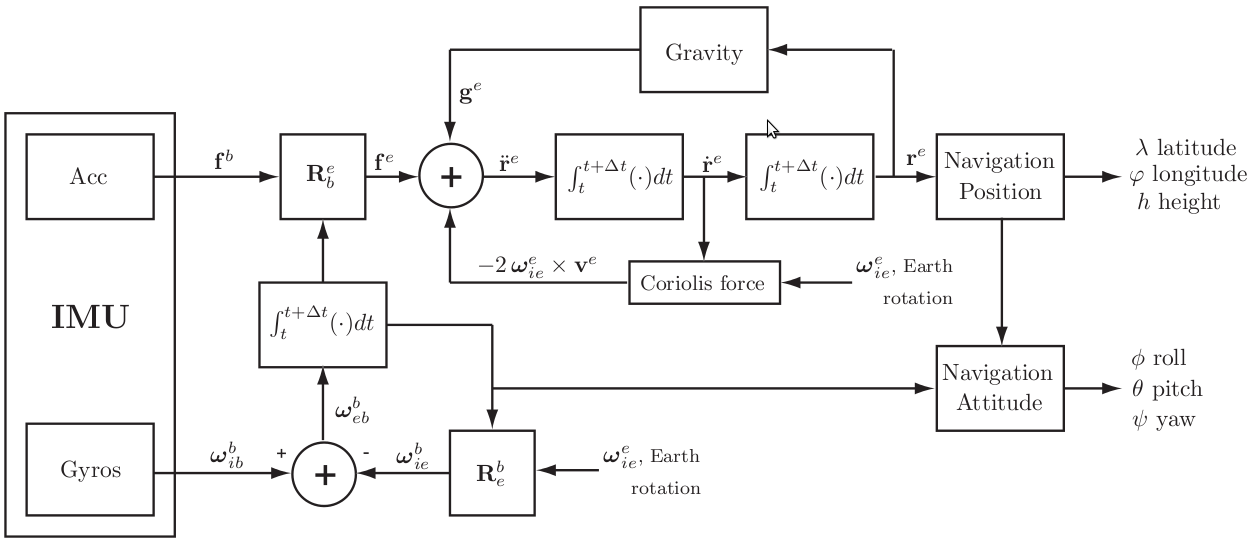
\includegraphics[scale=0.6]{sdins_algorithm}
\caption{Алгоритм роботи БІНС}
\label{fig:sdins}
\end{figure} 
Сигнали $\omega_{x,y,z}$ з виходу аналітичного компенсатора похибок використовуються 
для обчислення параметрів матриці напрямних  косинусів \textit{В}, яка визначає зв'язок 
між двома системами координат. Оскільки матриця напрямних  косинусів \textit{В} визначається 
між зв'язаними з ЛА осями й осями обертової навігаційної системи координат, то при 
розрахунках параметрів матриці \textbf{В }необхідно залучити обчислені проекції вектора 
кутової швидкості навігаційної системи координат, що відображено на схемі додатковими 
зв'язками, які враховують кутову швидкість, що виникає при обльоті сферичної Землі (
$\dot{\lambda }$, $\dot{h}$, $\dot{\varphi }$, і кутову швидкість обертання самої 
Землі $(\Omega_{\text{З}} )$.

Перетворення складових уявного прискорення $a_{x,y,z}$  від осей ЛА до осей навігаційної 
системи координат здійснюється за допомогою матриці напрямних  косинусів \textit{В}. Навігаційний 
обчислювач вирішує задачі, властиві всім платформним системам, оскільки на вході 
цього обчислювача сформовані проекції уявного прискорення на осі навігаційної системи 
координат і нічого принципово нового в розв'язанні цієї задачі немає. На виході БІНС 
формуються радіус-вектор місця розташування ЛА, вектор швидкості, а також кути орієнтації 
ЛА. 

В окремому випадку, коли за навігаційний базис вибраний горизонтальний орієнтований 
за сторонами світу тригранник, на виході системи будуть сформовані географічні (геодезичні) 
координати радіуса-вектора місця розташування $\lambda$, $\varphi$, \textit{H}, проекції 
відносної швидкості руху $V_N$, $V_E$, $V_H$, а також 
кути орієнтації ЛА в географічній системі координат -- справжній курс $\psi$, тангаж $\vartheta$ і 
крен $\gamma$. 

Обсяг обчислень у БІНС значний. Це пояснюється в основному тим фактом, що БЦОМ розв'язує 
задачі, які пов'язані з динамікою обертання ЛА, а також з динамікою поступального 
руху ЛА. Поступальні швидкості ЛА відносно малі. Наприклад, швидкість при польоті 
ЛА в напрямку на північ 1100 км/год відповідає швидкості зміни широти усього на 10 
град/год.

Таким чином, інтегрування для одержання швидкості і місця розташування можуть здійснюватися 
досить точно з використанням дуже простих методів чисельного інтегрування при низькій 
частоті повторення   в типовому випадку 10...20 Гц .

Кутові швидкості ЛА в типовому випадку за величиною на кілька порядків більші поступальних 
швидкостей. Зокрема, для маневрених ЛА кутові швидкості обертання можуть складати 
сотні градусів за секунду. В результаті цього інтегрування кутового положення в БІНС 
зв'язано з жорсткими вимогами до БЦОМ.

Оскільки для забезпечення високої точності інерціальної навігації потрібно, щоб похибки 
інтегрування кутового положення обмежувалися декількома частками кутової хвилини, 
необхідно застосовувати алгоритми інтегрування більш високого порядку при типових 
частотах повторення  80...50 Гц. 

З огляду на вище сказане, наведемо  варіант побудови алгоритмів БІНС для випадку, 
коли за навігаційний базис вибраний горизонтальний орієнтований за сторонами світу 
тригранник.
\vspace{5mm}

\textbf{Алгоритми БІНС, яка працює в географічній системі координат}

За навігаційний тригранник візьмемо тригранник \textit{NHE}, зв'язаний з земною поверхнею.
\begin{figure}[here]
\centering
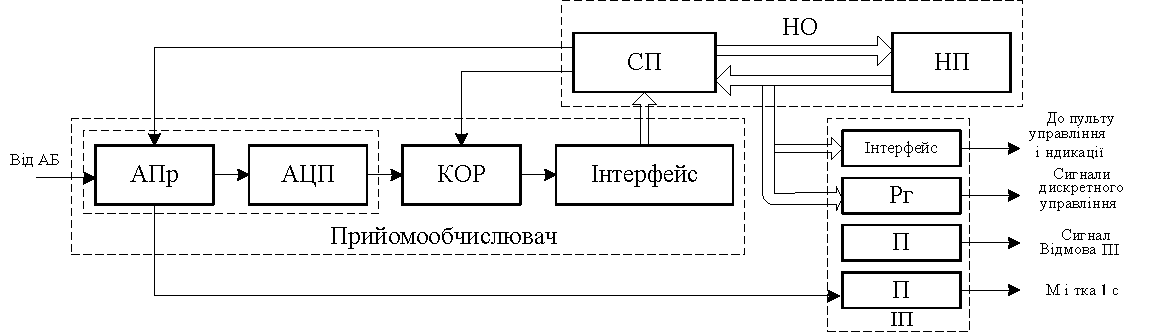
\includegraphics[scale=0.9]{sns}
\caption{Системи координат}
\label{fig:coordinat}
\end{figure} 
Виберемо наступний напрямок осей   \textit{NHE} (рис. \ref{fig:earth}):
\begin{ESKDexplanation}
\item \textit{OH} --збігається з вертикаллю;
\item \textit{ON} -- дотична до меридіана;
\item \textit{ОЕ} -- утворює праву трійку.
\end{ESKDexplanation}
В алгоритмах БІНС, зазвичай, виділяють динамічні та кінематичні рівняння. 
Динамічні рівняння реалізують трикомпонентну схему БІНС, у якій географічні координати  $\lambda$, 
$\varphi$,\textit{Н} визначаються інтегруванням рівнянь вигляду

\[\begin{array}{l} 
{\dot{\lambda}=\frac{V_{E} }{(R_{2} +H)\cos \varphi} ;} \\ 
{\dot{\varphi}=\frac{V_{N} }{R_{1} +H} ;} \\ 
{\dot{H}=V_{H,} } 
\end{array}\] 
\begin{ESKDexplanation}
\item де  $V_{N}$,$V_{E}$ -- північна та східна проекції шляхової швидкості 
(проекції на осі  системи координат \textit{NHE}  (див. рис. \ref{fig:earth}); 
\item $R_1$, \textit{R}2 -- два радіуси кривизни земного сфероїда (еліпсоїда обертання); 
\item $R_1$ -- радіус кривизни меридіонального перетину еліпсоїда (площиною \textit{HN}); 
\item $R_2$  -- радіус кривизни перетину еліпсоїда площиною \textit{HЕ} (площиною першого вертикала); 
\end{ESKDexplanation}
\[R_{1} =\frac{a(1-e^{2})}{(1-e^{2} \sin(\varphi)^{2})^{\frac{3}{2}} };\\
R_{2} =\frac{a}{\sqrt{1-e^{2} \sin(\varphi)^{2} } }.\] 
\begin{ESKDexplanation}
\item де\textit{ a}  --- велика піввісь  еліпсоїда (\textit{a }=  6378388 м); 
\item \textit{e} --- ексцентриситет еліпсоїда  ($e^{2} = 6,73 10^{-3}$);  
\item \textit{Н}  --- висота польоту. 
\end{ESKDexplanation}
Тут можна застосовувати такі ж спрощення, що й у платформних інерціальних системах. 
Зокрема, функції   $\frac{1}{R_{1} +H}$ та $\frac{1}{R_{2} +H} $ 
з точністю до членів порядку малості $10^{-5}$ можна представити 
в наступному вигляді:

\[\begin{array}{l} 
{\frac{1}{R_{1} +H} =\frac{1}{a} [1-e^{2} -\frac{H}{a} 
-\frac{3}{2} e^{2} \sin ^{2} \varphi-2e^{2} \frac{H}{a} +3e^{2} \frac{H}{a} \sin 
^{2} \varphi + (\frac{H}{a} )^{2} +}\\
{+e^{4} (1-3\sin ^{2} B+\frac{3}{8}\sin ^{4} \varphi);} \\ 

{\frac{1}{R_{2} +H} =\frac{1}{a}[1-\frac{H}{a} 
-\frac{1}{2} e^{2} \sin ^{2} \varphi+(\frac{H}{a})^{2} +e^{2} \frac{H}{a} 
\sin ^{2} \varphi+} \\ 
{+e^{4}(\frac{1}{4} \sin ^{2} \varphi-\frac{3}{8})\sin ^{2} \varphi]} 
\end{array}\] 
Якщо у формулах $\frac{1}{R_{1} +H}$ та $\frac{1}{R_{2} +H}$ 
зберегти лише члени порядку малості $10^{-2}$ , то вони приймуть 
вигляд

\begin{equation} 
\label{eq:elips} 
\begin{array}{l} 
{\frac{1}{R_{1} +H} \approx \frac{1}{a}[1-e^{2} -\frac{H}{a} -\frac{3}{2} e^{2} \sin(B)^{2}];} \\ 
{\frac{1}{R_{2} +H} \approx \frac{1}{a}[1-\frac{H}{a} -\frac{1}{2} e^{2} \sin(\varphi)^{2}].} 
\end{array} 
\end{equation} 
Слід відзначити, що використання спрощень \eqref{eq:elips} може призвести 
до похибок, порівняних з похибками високоякісних гіроскопічних вимірників, які використовуються 
в БІНС.

Складові шляхової швидкості ЛА  $V_E$ , $V_N$ , $V_H$  одержують в результаті інтегрування 
проекцій сигналів акселерометрів, виключаючи із них  складові коріолісового прискорення  і 
прискорення сили ваги: 
\begin{equation} 
\label{eq:Vi} 
 \begin{array}{l} 
{\dot{V}_{E} =a_{E} -(V_{N} \omega_{H_{\Sigma } } -V_{H} \omega_{N_{\Sigma} } )+g_{E} ;} \\ 
{\dot{V}_{H} =a_{H} -(V_{E} \omega_{N_{\Sigma } } -V_{N} \omega_{E_{\Sigma} } )+g_{H} ;} \\ 
{\dot{V}_{N} =a_{N} -(V_{H} \omega_{E_{\Sigma } } -V_{E} \omega_{H_{\Sigma} } )+g_{N} ,} 
\end{array}
\end{equation} 
\begin{ESKDexplanation}
\item де $a_{E,H,N} $ -- проекції уявного прискорення ЛА, вимірювані акселерометрами, 
на осі навігаційного тригранника; 
\item $g_{E,H,N} $ --- проекції вектора прискорення 
сили ваги, які враховують прискорення земного тяжіння, і прискорення, що викликається 
відцентровою силою інерції і зв'язане з обертанням Землі; 
\item складові в дужках --- проекції коріолісового прискорення на осі навігаційного тригранника; 
\item $\omega_{E_{\Sigma}}$, $\omega_{H_{\Sigma}}$, $\omega_{N_{\Sigma}}$ --- проекції кутової 
швидкості навігаційного тригранника відносно інерціального простору, які враховують 
проекції кутової швидкості обертання Землі $\Omega_{E}$, $\Omega_{H}$, $\Omega_{N}$ 
і складові відносної кутової швидкості навігаційного тригранника, які обумовлені 
рухом ЛА відносно Землі $\omega_{E_{V} }$, $\omega_{H_{V} }$, $\omega_{N_{V}}$: 
\end{ESKDexplanation}
\[\omega_{N_{\Sigma } } =\omega_{N_{V} } +2\Omega_{N} ;\\ 
\omega_{H_{\Sigma } } =\omega_{H_{V} } +2\Omega_{H} ;\\
\omega_{E_{\Sigma } } =\omega_{E_{V} } +2\Omega_{E} .\] 

У свою чергу, складові відносної кутової швидкості навігаційного тригранника і швидкості 
обертання Землі визначаються співвідношеннями
\[\begin{array}{l} 
{\omega_{E_{V}} =-\frac{V_{N} }{R_{1} +H} =-\dot{\varphi};} \\ 
{\omega_{H_{V}} =\frac{V_{E}}{(R_{2} +H)} tg\varphi=\dot{\lambda}\sin \varphi;} \\ 
{\omega_{N_{V}} =\frac{V_{E} }{(R_{2} +H)} =\dot{\lambda}\cos \varphi;} \end{array}\] 

\[\Omega_{N} =\Omega_{\text{З}}\cos \varphi;
\Omega_{H} =\Omega_{\text{З}}\sin \varphi; 
\Omega_{E} =0,\] 

\begin{ESKDexplanation}
 \item де  $\Omega_{\text{З}} $ --- кутова швидкість обертання Землі ($\Omega_{\text{З}}=7,27 \cdot 10^{-5}$ рад/с).
\end{ESKDexplanation}

Детермінована математична модель прискорення сили ваги існує тільки для нормальної 
складової поля сили ваги, що відповідає земному еліпсоїду з рівномірним розподілом 
мас в об'ємі цієї фігури. Градієнт цього поля в будь-якій точці, що належить поверхні 
еліпсоїда, спрямований за нормаллю до неї і розташований у площині меридіонального 
перетину. Оскільки точка місцеположення ЛА не належить поверхні Землі, то вектор 
градієнта нормального поля сили ваги $\bar{g}$ в цій точці не буде спрямований за 
лінією нормалі, опущеної з неї до поверхні земного еліпсоїда (вісь \textit{ОН}). 
Разом з тим, цей вектор буде розташований у площині меридіана точки \textit{О}, тобто 
в площині \textit{NOH. }Тоді, використовуючи  потенційну функцію нормального поля 
тяжіння земного сфероїда, з точністю до членів порядку малості $10^{-5}$  співвідношення 
для проекцій складових поля сили ваги $\bar{g}$ мають такий вигляд:
\[\begin{array}{l} 
{g_{E} =0;} \\
{g_{N} =\frac{1}{2} g[\frac{H}{a} (e^{2} -5q)+qe^{2} \sin^{2}\varphi]\sin^2\varphi;}\\
{g_{H} =-g\left\{1-2\frac{H}{a} -\right. (e^{2} +2q-3\frac{H}{a})
\frac{H}{a} +\left[\frac{1}{2} (5q-e\right. ^{2} )-\frac{1}{8} e^{4} +\frac{17}{18}qe^{2} +} \\ 
{ +(3e^{2} - 5q)\frac{H}{a} ]\sin ^{2} B-\frac{1}{2} qe^{2} \sin ^{4} \varphi+\frac{1}{16} e^{2} 
(\frac{1}{2} e^{2} -7q)\sin ^{2} 2\varphi\},} 
\end{array}\]
\begin{ESKDexplanation}
\item де \textit{g}= 9,78049 м/с2 прискорення сили ваги на екваторі; 
\item \textit{q} = $\Omega_{\text{З}}^{2} $ \textit{a/g} = 0,00346775 --- відношення 
відцентрової сили, обумовленої обертанням Землі, до сили ваги на екваторі. 
\end{ESKDexplanation}

З точністю до величин порядку малості $10^{-4}$ співвідношення для проекцій складових 
поля сили ваги $\bar{g}$ декілька спрощуються:

\[\begin{array}{l} 
{ g_{E} =0;} \\ 
{g_{N} =g\sin 2\varphi+\frac{5}{2} q\sin ^{2} B\frac{H}{a}(\frac{e^{2} }{2} -2q);} \\ 
{g_{H} =-g\left[1-\frac{e^{2} }{2}\sin ^{2} \varphi+\frac{3}{2} q\sin ^{2} \varphi+e^{4}(-\frac{1}{8} \sin ^{2} \varphi+\frac{1}{32} 
\sin ^{2} 2\varphi\right)+} \\ 
{ +e^{2} q\left(-\frac{17}{28} 
\sin ^{2} \varphi-\frac{5}{16} \sin ^{2} 2\varphi\right)+\frac{H}{a} e^{2} (3\sin ^{2} \varphi-1)+}\\ 
{ +\frac{Hq}{a} (-1-6\sin ^{2}\varphi)-2\frac{H}{a} +3\frac{H^{2} }{a^{2} }],} 
\end{array}\] 

а при малих значеннях висоти ($Н\leq$ 100 км ) проекції вектора  $\bar{g}$ на 
осі \textit{NHE}, якщо в них зберегти лише члени порядку малості $10^{-2}$, 
взагалі мають простий вигляд: 
\[\begin{array}{l} 
{g_{E} =0;}\\
{g_{N} =0;}\\ 
{g_{H} =-g(1+5,2884\cdot 10^{-3} \sin ^{2}\varphi)[1-\frac{2H}{a}
(1-e\sin^{2}\varphi )]} 
\end{array}\] 
Є й інші форми запису даної складової.

При розв'язанні кінематичних рівнянь розраховуються проекції $a_{E,H,N} $ уявного 
прискорення ЛА на осі навігаційного тригранника \textit{NHE}за показаннями акселерометрів 
зі зв'язаної з ЛА системи координат \textit{XYZ} з використанням матриці напрямних  
косинусів \textbf{В}
\[ \left[\begin{array}{c} 
{a_{N} } \\ 
{a_{H} } \\ 
{a_{E} }
\end{array}\right]=B
\left[\begin{array}{c} 
{a_{x_{\text{ЛА}} } } \\ 
{a_{y_{\text{ЛА}} } } \\ 
{a_{z_{\text{ЛА}} } } 
\end{array}\right]\] 
Матриця напрямних  косинусів  має такий вигляд:
\[B=\left[\begin{array}{c|c|c} 
{\cos \psi \cos \vartheta } & 
{\sin \psi \sin \gamma -\cos \psi \sin \vartheta \cos \gamma } & 
{\sin \psi \cos \gamma +\sin \gamma \sin \vartheta \cos \psi } \\  \hline {\sin \vartheta } & 
{\cos \vartheta \cos \gamma} & 
{-\cos \vartheta \sin \gamma } \\  \hline {-\sin \psi \cos \vartheta } & 
{\cos \psi \sin \gamma +\sin \psi \sin \vartheta \cos \gamma } & 
{\cos \psi \cos \gamma -\sin \psi \sin \vartheta \sin \gamma } 
\end{array}\right]\] 
\begin{ESKDexplanation}
\item де $\gamma$, $\vartheta$, $\psi$ -- кути крену, тангажа і рискання. Кут рискання 
відрізняється від географічного курсу $\psi$г знаком, тобто $\psi$г = $\psi$.
\end{ESKDexplanation}
Матриця напрямних  косинусів \textbf{В} може бути отримана в різні способи. Наведемо приклади 
деяких з них. 

Знайти матрицю \textbf{В} можна в результаті розв'язання 
узагальненого рівняння Пуассона за інформацією про кутову швидкість ЛА відносно інерціального 
простору $\omega_{\text{ЛА}}$ і кутову швидкість навігаційної системи координат відносно 
інерціального простору $\omega_{NHE}$, яка враховує кутову швидкість 
обертання Землі і кутову швидкість, обумовлену обльотом ЛА сферичної Землі 
\[  \dot{B}=B\omega_{\text{ЛА}} -\omega_{NHE}B\] 
де 
\[\omega_{\text{ЛА}} =\left[\begin{array}{ccc} 
{0} & {-\omega_{z_{\text{ЛА}} } } & {\omega_{y_{\text{ЛА}}}} \\ 
{\omega_{z_{\text{ЛА}} } } & {0} & {-\omega_{x_{\text{ЛА}}}} \\ 
{-\omega_{y_{\text{ЛА}} } } & {\omega_{x_{\text{ЛА}} } } & {0} 
\end{array}\right];\]\\
\[\omega_{NHE} =\left[\begin{array}{ccc} 
{0} & {-(\omega_{E_{V} } +\Omega_{E} )} & {(\omega_{H_{V} } +\Omega_{H} )} \\ 
{(\omega_{E_{V} } +\Omega_{E})} & {0} & {-(\omega_{N_{V} } +\Omega_{N} )} \\ 
{-(\omega_{H_{V} } +\Omega_{H})}& {(\omega_{N_{V} } +\Omega_{N} )} & {0} 
\end{array}\right];\] 
\begin{ESKDexplanation}
  \item $\omega_{x_{\text{ЛА}}}$, $\omega_{y_{\text{ЛА}}}$, $\omega_{z_{\text{ЛА}}}$  -- кутові 
  швидкості ЛА відносно зв'язаних осей, вимірювані датчиками кутової швидкості; 
  \item $\omega_{E_{V} }$, $\omega_{H_{V} }$, $\omega_{N_{V}}$ були визначені раніше.
\end{ESKDexplanation}
За елементами матриці  \textit{B} визначаються кути орієнтації ЛА: крен $\gamma$, тангаж 
$\vartheta$ рискання (курс) $\psi $: 
\begin{equation} 
\label{eq:angels} 
\begin{array}{l} 
{\gamma ={\rm arctg}\left(
\frac{-b_{23} }{b_{22} } \right)={\rm arcsin}\left(\frac{-b_{23} }{\sqrt{1-b_{21}^{2} 
} } \right)={\rm arccos}\left(\frac{b_{22} }{\sqrt{1-b_{21}^{2} } } \right)\; ; 
} \\ 
{\vartheta ={\rm arctg}\left(\frac{b_{21} }{\sqrt{b_{22}^{2} +b_{33}^{2} } } 
\right){\rm \; }={\rm arcsin(}b_{21} {\rm )}={\rm arccos}\left(\sqrt{1-b_{21}^{2} 
} \right)} \\ 
{\psi =-{\rm arctg}\left(\frac{b_{31} }{b_{11} } \right)={
\rm arcsin}\left(\frac{-b_{31} }{\sqrt{1-b_{21}^{2} } } \right)={\rm arccos}\left(
\frac{b_{11} }{\sqrt{1-b_{21}^{2} } } \right).} 
\end{array} 
\end{equation} 
Інший алгоритм отримання матриці напрямних косинусів припускає її  формування безпосередньо 
за кутами  $\gamma$, $\vartheta$, $\psi$. 
\begin{figure}[here]
\centering
%\includegraphics[scale=0.9]{earth}
\caption{Системи координат}
\label{fig:kinemat}
\end{figure} 
Кінематичні співвідношення між кутами $\gamma$, $\vartheta$, $\psi$ і проекціями вектора абсолютної кутової 
швидкості на осі зв'язаної системи координат $\omega_{x_{\Sigma } }$ , $\omega_{y_{\Sigma }}$, 
$\omega_{z_{\Sigma}} $ можна одержати з рис. \ref{fig:kinemat}, 
на якому показано перетворення навігаційної системи координат \textit{OLR$\Phi $ }у 
зв'язану \textit{OXYZ} шляхом трьох поворотів: \textit{1}   навколо осі \textit{OR}; \textit{2}  
навколо проміжної осі \textit{OZ*}; \textit{3}  навколо осі \textit{OX}.

 Звичайно, що кутові швидкості $\dot{\psi }$, $\dot{\vartheta }$, $\dot{\gamma }$, 
які спрямовані уздовж відповідних осей, є складовими абсолютної кутової швидкості 
ЛА.

 Проектуючи $\dot{\psi }$,$\dot{\vartheta }$, $\dot{\gamma }$на осі зв'язаної системи 
координат, отримаємо:

\[\begin{array}{l} 
{\omega_{x_{\Sigma } } =\dot{\gamma }+\dot{\psi }\sin \vartheta ;} \\ 
{\omega_{y_{\Sigma } } =\dot{\vartheta }\sin \gamma +\dot{\psi}\cos \vartheta\cos \gamma ;} \\ 
{\omega_{z_{\Sigma } } =\dot{\vartheta }\cos \gamma -\dot{\psi}\cos \vartheta \sin \gamma .} 
\end{array}\] 
Розв'язуючи ці співвідношення, одержимо такі кінематичні рівняння:
\[\begin{array}{l} 
{\dot{\psi }=(\omega_{y_{\Sigma } } \cos \gamma -\omega_{z_{\Sigma }} \sin \gamma)\sec \vartheta ;} \\ 
{\dot{\gamma }=\omega_{x_{\Sigma } } +tg\vartheta (\omega_{z_{\Sigma } } \sin \gamma -\omega_{y_{\Sigma } } \cos \gamma );} \\ 
{\dot{\vartheta }=\omega_{y_{\Sigma } } \sin \gamma +\omega_{z_{\Sigma }} \cos \gamma.} 
\end{array}\] 
У свою чергу 
\[ \begin{array}{l} 
  {\omega_{y_{\Sigma } } =\omega_{y_{\text{ЛА}} } -\omega_{y_{_{NHE}}};} \\ 
  {\omega_{x_{\Sigma } } =\omega_{x_{\text{ЛА}}}  -\omega_{x_{NHE}} ;} \\ 
  {\omega_{z_{\Sigma } } =\omega_{z_{\text{ЛА}}}  -\omega_{z_{NHE}}.} \end{array}\] 
\begin{ESKDexplanation}
\item де $\omega_{y_{\text{ЛА}}}$,$\omega_{x_{\text{ЛА}}}$,$\omega_{z_{\text{ЛА}}}$ -- проекції 
кутової швидкості ЛА відносно інерціального простору на осі зв'язаної системи координат, 
вимірювані датчиками кутових швидкостей;
\item $\omega_{y_{_{NHE}}}$,$\omega_{x_{_{NHE}}}$,$\omega_{z_{_{NHE}}}$  -- проекції кутової швидкості навігаційного тригранника 
відносно інерціального простору на осі зв'язаної системи координат, які враховують 
проекції кутової швидкості обертання Землі  $\Omega_{H}$,$\Omega_{E}$ ,$\Omega_{N}$
і складові відносної кутової швидкості навігаційного тригранника, 
що обумовлені рухом ЛА відносно Землі $\omega_{H_{V}}$ , $\omega_{E_{V}}$ ,
$\omega_{N_{V}} $. 
\end{ESKDexplanation}
% \includegraphics[bb=0mm 0mm 208mm 296mm, width=36.3mm, height=6.6mm, viewport=3mm 
% 4mm 205mm 292mm]{image1.eps} 
Ці проекції кутової швидкості визначаються в результаті 
розв'язання матричного рівняння 
\[\left
[\begin{array}{c} {\omega_{x_{NHE} } } \\ 
{\omega_{y_{NHE} } } \\ 
{\omega_{z_{NHE} } } 
\end{array}\right]
=B^{T} 
\left[\begin{array}{c} {\omega_{N_{V} 
} +\Omega_{N} } \\ 
{\omega_{H_{V} } +\Omega_{H} } \\ 
{\omega_{E_{V} } +\Omega_{E} } 
\end{array}\right] .\] 
Перевагою такого підходу до визначення кутів орієнтації ЛА (інтегруванням диференціальних 
рівнянь, що описують швидкості зміни кутів Ейлера, а не за арктангенсами відношення 
елементів матриці напрямних  косинусів) є відсутність обмежень $\gamma$ $\pm90^{o}$, 
що особливо важливо при визначенні курсу ЛА на віражах. 

Тривимірні матриці напрямних  косинусів досить зручні для обчислень у бортовій ЦОМ. 
Однак формування матриці \textbf{В} з використанням тригонометричних функцій вимагає 
значних обчислювальних витрат. 

Для визначення орієнтації ЛА можна використовувати не тільки напрямні косинуси, але 
і параметри Родрига-Гамільтона у формі кватерніонів. Достоїнство методу кватерніонів 
полягає в тому, що він дозволяє описувати перехід від однієї системи координат до 
іншої за допомогою всього лише чотирьох чисел, а не 9 напрямних  косинусів.

Кватерніонний метод ґрунтується  на теоремі Ейлера, яка доводить, що будь-який поворот 
однієї системи координат відносно іншої можна подати, як поворот на деякий кут навколо 
однієї нерухомої осі.

Кватерніон є компактною формою запису орієнтації зазначеної осі (векторна частина 
кватерніона $\lambda_{1} ,\lambda_{2} ,\lambda_{3} $) і кута повороту (скалярна 
частина кватерніона $\lambda_{0} $) відповідно до теореми Ейлера.

Застосування кватерніонів дозволяє подати ортогональні перетворення у формі множення 
кватерніонів. Дії над кватерніонами допускають матричні операції з використанням 
симетризованих матриць, що дуже зручно при створенні програм бортових обчислювачів. 

Відповідно 
до теореми Ейлера-Шаля усяке переміщення твердого тіла, яке має нерухому точку, можна 
зобразити як результат повороту навколо незмінного напрямку (ейлерової осі) на певний 
кут $\varphi $. Якщо зв'язати з розглянутим твердим тілом правий ортогональний координатний 
тригранник, то параметри Родрига-Гамільтона $\lambda_{0}$ ,$\lambda_{1}$, $\lambda_{2}$,
$\lambda_{3}$ ,що однозначно характеризують згадані переміщення, можна задати 
такими виразами: 
\[\lambda_{1} =\frac{l_{1} \sin \varphi }{2};
  \lambda_{2} =\frac{l_{2} \sin \varphi }{2};
  \lambda_{3} =\frac{l_{3} \sin \varphi }{2};
  \lambda_{0} =\frac{\cos \varphi }{2} ,\] 
\begin{ESKDexplanation}
 \item де $l_{1} ,l_{2} ,l_{3} -$косинуси кутів, утворених ейлеровою віссю з осями тригранника 
в його вихідному та кінцевому положенні. 
\end{ESKDexplanation}

Зв'яжемо з ЛА, на якому встановлена БІНС, ортонормований базис \textbf{Е} -- 
праву трійку взаємно ортогональних одиничних 
векторів $e_{1}$ ,$e_{2}$ ,$e_{3}$. Орієнтацію базису \textbf{Е} відносно ортонормованого 
інерціального базису \textbf{І}, складеного з ортів $i_{1}$ ,$i_{2}$ ,$i_{3}$ , охарактеризуємо 
параметрами Родрига-Гамільтона $\lambda_{0}$ ,$\lambda_{1}$ ,$\lambda_{2}$ ,$\lambda 
_{3}$. Матриця напрямних  косинусів, що обчислена за параметрами Родрига-Гамільтона 
(кватерніонами), має такий вигляд:

\[B=\left|
\begin{array}{ccc} {1-2(\lambda_{2}^{2} +\lambda_{3}^{2} )} & 
{2(\lambda_{1} \lambda_{2} -\lambda_{0} \lambda_{3} )} & 
{2(\lambda_{1} \lambda_{3} +\lambda_{0} \lambda_{2} )} \\ 
{2(\lambda_{1} \lambda_{2} +\lambda_{0} \lambda_{3} )} & 
{1-2(\lambda_{1}^{2} +\lambda_{3}^{2} )} & 
{2(\lambda_{2} \lambda_{3} -\lambda_{0} \lambda_{1} )} \\ 
{2(\lambda_{1} \lambda_{3} -\lambda_{0} \lambda_{2} )} & 
{2(\lambda_{2} \lambda_{3} +\lambda_{0} \lambda_{1} )} & 
{1-2(\lambda_{1}^{2} +\lambda_{2}^{2} )} \end{array}\right|.\] 

Вимірники кутової швидкості, що входять до складу БІНС, вимірюють координати 
$\omega_{x}$, $\omega_{y}$, $\omega_{z}$ вектора $\bar{\Omega }$ абсолютної кутової швидкості 
базису \textbf{Е}, що задані в цьому базисі. Необхідно, знаючи значення параметрів 
Родрига-Гамільтона в момент часу $t=t_{0} $ і використовуючи сигнали вимірників кутової 
швидкості, обчислювати параметри Родрига-Гамільтона при $t>t_{0} $. У початковий 
момент часу за інформацією про кути крену тангажа і курсу можна розрахувати вихідні 
значення параметрів Родрига-Гамільтона: 
\[\begin{array}{l} 
{\lambda_{0_{0} } =\sin  \left({\gamma_{0}  \mathord{
\left/{\vphantom{\gamma_{0}  2}}\right.\kern-\nulldelimiterspace} 2} \right)\sin 
 \left({\vartheta_{0}  \mathord{\left/{\vphantom{\vartheta_{0}  2}}\right.\kern-
\nulldelimiterspace} 2} \right)\sin  \left({\psi_{0}  \mathord{\left/{\vphantom{
\psi_{0}  2}}\right.\kern-\nulldelimiterspace} 2} \right)+\cos  \left({\gamma 
_{0}  \mathord{\left/{\vphantom{\gamma_{0}  2}}\right.\kern-\nulldelimiterspace} 
2} \right)\cos  \left({\vartheta_{0}  \mathord{\left/{\vphantom{\vartheta_{0}  
2}}\right.\kern-\nulldelimiterspace} 2} \right)\cos  \left({\psi_{0}  \mathord{
\left/{\vphantom{\psi_{0}  2}}\right.\kern-\nulldelimiterspace} 2} \right);} \\ 

{\lambda_{1_{0} } =-\sin  \left({\vartheta_{0}  \mathord{\left/{\vphantom{
\vartheta_{0}  2}}\right.\kern-\nulldelimiterspace} 2} \right)\sin  \left({\psi 
_{0}  \mathord{\left/{\vphantom{\psi_{0}  2}}\right.\kern-\nulldelimiterspace} 2} 
\right)\cos  \left({\gamma_{0}  \mathord{\left/{\vphantom{\gamma_{0}  2}}\right.
\kern-\nulldelimiterspace} 2} \right)+\sin \left({\gamma_{0}  \mathord{\left/{\vphantom{
\gamma_{0}  2}}\right.\kern-\nulldelimiterspace} 2} \right)\cos  \left({\vartheta 
_{0}  \mathord{\left/{\vphantom{\vartheta_{0}  2}}\right.\kern-\nulldelimiterspace} 
2} \right)\cos  \left({\psi_{0}  \mathord{\left/{\vphantom{\psi_{0}  2}}\right.
\kern-\nulldelimiterspace} 2} \right);} \\ 

{\lambda_{2_{0} } =\sin \left({
\gamma_{0}  \mathord{\left/{\vphantom{\gamma_{0}  2}}\right.\kern-\nulldelimiterspace} 
2} \right)\cos  \left({\vartheta_{0}  \mathord{\left/{\vphantom{\vartheta_{0}  
2}}\right.\kern-\nulldelimiterspace} 2} \right)\sin  \left({\psi_{0}  \mathord{
\left/{\vphantom{\psi_{0}  2}}\right.\kern-\nulldelimiterspace} 2} \right)+\sin 
 \left({\vartheta_{0}  \mathord{\left/{\vphantom{\vartheta_{0}  2}}\right.\kern-
\nulldelimiterspace} 2} \right)\cos  \left({\gamma_{0}  \mathord{\left/{\vphantom{
\gamma_{0}  2}}\right.\kern-\nulldelimiterspace} 2} \right)\cos  \left({\psi_{0}  
\mathord{\left/{\vphantom{\psi_{0}  2}}\right.\kern-\nulldelimiterspace} 2} \right);}\\ 

{\lambda_{3_{0} } =\sin  \left({\psi_{0}  \mathord{\left/{\vphantom{
\psi_{0}  2}}\right.\kern-\nulldelimiterspace} 2} \right)\cos  \left({\gamma_{0}  
\mathord{\left/{\vphantom{\gamma_{0}  2}}\right.\kern-\nulldelimiterspace} 2} \right)
\cos  \left({\vartheta_{0}  \mathord{\left/{\vphantom{\vartheta_{0}  2}}\right.
\kern-\nulldelimiterspace} 2} \right)-\sin  \left({\gamma_{0}  \mathord{\left/{
\vphantom{\gamma_{0}  2}}\right.\kern-\nulldelimiterspace} 2} \right)\sin  \left({
\vartheta_{0}  \mathord{\left/{\vphantom{\vartheta_{0}  2}}\right.\kern-\nulldelimiterspace} 
2} \right)\cos  \left({\psi_{0}  \mathord{\left/{\vphantom{\psi_{0}  2}}\right.
\kern-\nulldelimiterspace} 2} \right).} \end{array}\] 

Поточні значення параметрів $\lambda_{0}$ ,$\lambda_{1}$ ,$\lambda_{2}$ ,$\lambda_{3}$ можна 
визначити, знаючи проекції кутової швидкості ЛА $\omega_{x}$ ,$\omega_{y}$ ,$\omega_{z}$ 
на зв'язаній осі $XYZ$, шляхом розв'язання лінійного диференціального рівняння 
зі змінними коефіцієнтами. У цьому випадку параметри $\lambda_{0}$ ,$\lambda_{1}$ 
,$\lambda_{2}$ ,$\lambda_{3}$ кватерніона  описують  положення  осей ЛА  $XYZ$  відносно  
інерціального простору:

\[\dot{\lambda }=\frac{1}{2} \Omega(t)\cdot \lambda(t)\] 
\begin{ESKDexplanation}
\item де $\Omega(t)$ -- кососиметрична $(4\times 4)$-матриця, яка 
відповідає вектору $\omega =[\omega_{x} \omega_{y} \omega_{z}]^{T}  $
\end{ESKDexplanation}
\[\Omega (t)=\left[
\begin{array}{cccc} 
  {0} & {-\omega_{x}} & {-\omega_{y}} & {-\omega_{z}} \\ 
  {\omega_{x}} & {0} & {\omega_{z} } & {-\omega_{y}} \\ 
  {\omega_{y}} & {-\omega_{z}} & {0} & {\omega_{x}} \\ 
  {\omega_{z}} & {\omega_{y}} & {-\omega_{x}} & {0} 
\end{array}\right];
\lambda =\left[\begin{array}{c} 
  {\lambda_{0} } \\ 
  {\lambda_{1} } \\ 
  {\lambda_{2} } \\ 
  {\lambda_{3} } 
\end{array}
\right].\] 

Цей вираз є кватерніонним однорідним лінійним диференціальним рівнянням першого порядку 
зі змінним коефіцієнтом у вигляді гіперкомплексного числа з дійсною частиною, що 
дорівнює нулю. У скалярній формі це рівняння  має такий вигляд:

\[\begin{array}{l} 
{\dot{\lambda}_{0} =-0,5(\omega_{x} \lambda_{1} +\omega_{y} \lambda_{2} +\omega_{z} \lambda_{3} ;} \\ 
{\dot{\lambda}_{1} =-0,5(\omega_{x} \lambda_{0} +\omega_{z} \lambda_{2} +\omega_{y} \lambda_{3});} \\ 
{\dot{\lambda}_{2} =-0,5(\omega_{y} \lambda_{0} +\omega_{z} \lambda_{1} +\omega_{x} \lambda_{3});} \\ 
{\dot{\lambda}_{3} =-0,5(\omega_{z} \lambda_{0} +\omega_{y} \lambda_{1} +\omega_{x} \lambda_{2}).}
\end{array}\] 

Динаміка зміни параметрів кватерніона у випадку, коли кватерніон характеризує взаємне 
положення зв'язаних з ЛА осей $XYZ$ і обертових навігаційних осей \textit{NHE}, описується 
рівняннями
\begin{equation}
 \left[\begin{array}{c} 
{\dot{\lambda }_{0} } \\ 
{\dot{\lambda }_{1} } \\ 
{\dot{\lambda }_{2} } \\ 
{\dot{\lambda }_{3} } 
\end{array}\right]=\frac{1}{2} \left[\begin{array}{cccc}
{0} & {-\omega_{x\Sigma } } & {-\omega_{y\Sigma } } & {-\omega_{z\Sigma } } \\ 
{\omega_{x\Sigma } } & {0} & {\omega_{z\Sigma } } & {-\omega_{y\Sigma } } \\ 
{\omega_{y\Sigma } } & {-\omega_{z\Sigma } } & {0} & {\omega_{x\Sigma } } \\ 
{\omega_{z\Sigma } } & {\omega_{y\Sigma } } & {-\omega_{x\Sigma } } & {0} 
\end{array}
\right]\cdot 
\left[\begin{array}{c} 
{\lambda_{0} } \\ {\lambda_{1} } \\ {\lambda_{2} } \\ {\lambda_{3} } 
\end{array}\right] 
\label{eq:qdiff}
\end{equation}

\begin{ESKDexplanation}
 \item У свою чергу  

\[\omega_{x_{\Sigma } } =\omega_{x_{\text{ЛА}} } -\omega_{x_{NHE} } ;  \omega 
_{y_{\Sigma } } =\omega_{y_{\text{ЛА}} } -\omega_{y_{NHE} } ;  \omega_{z_{\Sigma 
} } =\omega_{z_{\text{ЛА}} } -\omega_{z_{NHE} } ,\] 

де  $\omega_{y_{\text{ЛА}}}$, $\omega_{x_{\text{ЛА}}}$, $\omega_{z_{\text{ЛА}}}$ --
проекції кутової швидкості ЛА відносно інерціального простору на осі 
зв'язаної системи координат, вимірювані датчиками кутових швидкостей;

 \item $\omega_{x_{NHE}} ,\omega_{y_{NHE}} ,\omega_{z_{NHE}} $ -- проекції кутової 
швидкості навігаційної системи координат відносно інерціального простору на осі зв'язаної 
системи координат, що визначаються в результаті розв'язання матричного рівняння 
\[\left[
\begin{array}{c} 
{\omega_{x_{NHE}} } \\ 
{\omega_{y_{NHE}} } \\ 
{\omega_{z_{NHE} }} 
\end{array}\right]=B^{T} 
\left[\begin{array}{c} 
{\omega_{N_{V}} +\Omega_{N}} \\ 
{\omega_{H_{V}} +\Omega_{H}} \\ 
{\omega_{E_{V}} +\Omega_{E}} 
\end{array}\right].\] 
\end{ESKDexplanation}
Ці складові розраховуються й у раніше розглянутих алгоритмах.


У скалярній формі рівняння \eqref{eq:qdiff} мають вигляд:
\[\begin{array}{l} 
{\dot{\lambda }_{0} =-0,5(\omega_{x\Sigma } \lambda_{1} +\omega_{y\Sigma } \lambda_{2} +\omega_{z\Sigma } \lambda_{3} );} \\ 
{\dot{\lambda }_{1} =-0,5(\omega_{x\Sigma } \lambda_{0} +\omega_{z\Sigma } \lambda_{2} +\omega_{y\Sigma } \lambda_{3} );} \\ 
{\dot{\lambda }_{2} =-0,5(\omega_{y\Sigma } \lambda_{0} +\omega_{z\Sigma } \lambda_{1} +\omega_{x\Sigma } \lambda_{3} );} \\ 
{\dot{\lambda }_{3} =-0,5(\omega_{z\Sigma } \lambda_{0} +\omega_{y\Sigma } \lambda_{1} +\omega_{x\Sigma } \lambda_{2} ).} 
\end{array}\] 
Матрицю \textit{В} перерахування зі зв'язаної в географічну систему координат можна 
також отримати шляхом перемножування двох матриць, з яких одна перераховує зі зв'язаних 
у інерціальні осі, друга -- з інерціальних у географічні. Кожна з двох матриць також 
обчислюється на основі параметрів Родрига-Гамільтона, які у свою чергу визначаються 
чисельним алгоритмом другого порядку, побудованим на основі методу послідовних наближень  
Пікара:
\[B=C^{T}A\]

\[A=\left| \begin{array}{ccc} 
{1-2(\lambda_{2}^{2} +\lambda_{3}^{2} )} & {2(\lambda_{1} \lambda_{2}-\lambda_{0} \lambda_{3})} & {2(\lambda_{1} \lambda_{3} +\lambda_{0}\lambda_{2} )} \\ 
{2(\lambda_{1} \lambda_{2} +\lambda_{0} \lambda_{3} )} & {1-2(\lambda_{1}^{2} +\lambda_{3}^{2} )} & {2(\lambda_{2} \lambda_{3} -\lambda_{0}\lambda_{1})} \\ 
{2(\lambda_{1} \lambda_{3} -\lambda_{0} \lambda_{2} )} & {2(\lambda_{2} \lambda_{3} +\lambda_{0} \lambda_{1} )} & {1-2(\lambda_{1}^{2} +\lambda_{2}^{2})} 
\end{array}  \right|;\]


\begin{equation}
\label{eq:qcalc} 
\begin{array}{cccc} 
{\lambda_{0}^{(k+1)}=\lambda_{0}^{(k)} -\lambda_{0}^{(k)} {e \mathord{/{\vphantom{e 8}}.\kern-\nulldelimiterspace} 8} 
-0,5(\lambda_{1}^{(k)} \Delta \beta_{x} +\lambda_{2}^{(k)} \Delta \beta_{y} +\lambda_{3}^{(k)} \Delta \beta_{z});}\\ 
{\lambda_{1}^{(k+1)} =\lambda_{1}^{(k)} -\lambda_{1}^{(k)} {e \mathord{/{\vphantom{e 8}}.\kern-\nulldelimiterspace} 8}
-0,5(\lambda_{0}^{(k)}\Delta \beta_{x} +\lambda_{3}^{(k)} \Delta \beta_{y} +\lambda_{2}^{(k)} \Delta\beta_{z});} \\ 
{\lambda_{2}^{(k+1)} =\lambda_{2}^{(k)} -\lambda_{2}^{(k)} {e \mathord{/{\vphantom{e 8}}.\kern-\nulldelimiterspace} 8} 
-0,5(\lambda_{3}^{(k)} \Delta \beta_{x} +\lambda_{0}^{(k)} \Delta \beta_{y}+\lambda_{1}^{(k)} \Delta \beta_{z} )  ;} \\ 
{\lambda_{3}^{(k+1)} =\lambda_{3}^{(k)} -\lambda_{3}^{(k)} {e \mathord{/{\vphantom{e 8}}.\kern-\nulldelimiterspace} 8} 
-0,5(\lambda_{2}^{(k)} \Delta \beta_{x} +\lambda_{1}^{(k)} \Delta \beta_{y} +\lambda_{0}^{(k)} \Delta \beta_{z} )  ,} 
\end{array} 
\end{equation}

\begin{ESKDexplanation}
\item де   $e=\Delta \beta_{x}^{2} +\Delta \beta_{y}^{2} +\Delta \beta_{z}^{2} ;$
\[\Delta \beta_{x} =\int_{t_{k} }^{t_{k} +1}\omega_{x_{\text{ЛА}} } dt ;   
 \Delta \beta_{y} =\int_{t_{k} }^{t_{k} +1}\omega_{y_{\text{ЛА}} } dt ;   
 \Delta \beta_{z} =\int_{t_{k} }^{t_{k} +1}\omega_{z_{\text{ЛА}} } dt ;\] 

\item $\Delta $$\beta $\textit{x}, $\Delta $$\beta $\textit{y}, $\Delta $$\beta $\textit{z }-- збільшення 
інтегралів від проекцій абсолютної кутової швидкості ЛА на осі чутливості гіроскопів 
(показання датчиків кутової швидкості БІНС, які вимірюють не проекції кутових швидкостей, 
а збільшення кутів повороту навколо своїх осей чутливості, тобто показання інтегруючих 
датчиків кутової швидкості):
\end{ESKDexplanation}
\[C=\left|\begin{array}{ccc} 
{1-2(\mu_{2}^{2} +\mu_{3}^{2} )} & {2(\mu_{1} \mu_{2} -\mu_{0} \mu_{3} )} & {2(\mu_{1} \mu_{3} +\mu_{0} \mu_{2} )} \\ 
{2(\mu_{1} \mu_{2} +\mu_{0} \mu_{3} )} & {1-2(\mu_{1}^{2} +\mu_{3}^{2} )} & {2(\mu_{2} \mu_{3} -\mu_{0} \mu_{1} )} \\ 
{2(\mu_{1} \mu_{3} -\mu_{0} \mu_{2} )} & {2(\mu_{2} \mu_{3} +\mu_{0} \mu_{1} )} & {1-2(\mu_{1}^{2} +\mu_{2}^{2} )} 
\end{array}  \right|;\] 

\[\begin{array}{l} 
{\mu_{0}^{(k+1)}=\mu_{0}^{(k)} -0,5\left(\mu_{1}^{(k)} \Omega_{x} +\mu_{2}^{(k)} \Omega_{y}+\mu_{3}^{(k)} \Omega_{z} \right) dt;}\\ 
{\mu_{1}^{(k+1)}=\mu_{1}^{(k)} -0,5\left(\mu_{0}^{(k)} \Omega_{x} +\mu_{3}^{(k)} \Omega_{y}+\mu_{2}^{(k)} \Omega_{z} \right) dt;} \\ 
{\mu_{2}^{(k+1)}=\mu_{2}^{(k)} -0,5\left(\mu_{3}^{(k)} \Omega_{x} +\mu_{0}^{(k)} \Omega_{y}+\mu_{1}^{(k)} \Omega_{z} \right) dt;} \\ 
{\mu_{3}^{(k+1)}=\mu_{3}^{(k)} -0,5\left(\mu_{2}^{(k)} \Omega_{x} +\mu_{1}^{(k)} \Omega_{y} +\mu_{0}^{(k)} \Omega_{z} \right) dt} 
\end{array}\] 

\begin{ESKDexplanation}
\item де $\Omega_{x} =\omega_{N_{V} } +\Omega_{N}$ ;  $\Omega_{y} =\omega_{H_{V} 
} +\Omega_{H}$ ;  $\Omega_{z} =\omega_{E_{V} } +\Omega_{E} $ -- проекції абсолютної 
кутової швидкості географічного базису на його осі .
\end{ESKDexplanation}
До переваг цього методу побудови матриці орієнтації відноситься гарантована ортогональність 
матриці орієнтації, обчисленої за співвідношеннями \eqref{eq:qcalc}. Крім цього, 
практика показує, що обчислення з використанням параметрів Родрига-Гамільтона дає 
найменші обчислювальні витрати в порівнянні з іншими методами за умови забезпечення 
однакових точностних характеристик. Разом з тим, визначення матриці \textit{В }через 
параметри Родрига-Гамільтона призводить до необхідності рішення двох однотипних систем 
лінійних диференціальних рівнянь четвертого порядку кожна.

За елементами матриці  \textbf{B} відповідно до \eqref{eq:angels} визначаються 
кути орієнтації ЛА:  крен $\gamma $, тангаж $\vartheta$ та рискання (курс) $\psi$: 

Після знаходження матриці \textit{В} система рівнянь для проведення навігаційних 
розрахунків замикається. 

Алгоритм проведення навігаційних розрахунків у випадку формування матриці напрямних  
косинусів безпосередньо за кутами  $\gamma$, $\vartheta$, $\psi$ можна представити 
у вигляді \eqref{eq:fgyro}\dots \eqref{eq:gravity}. У випадку недостатньої 
швидкодії бортового процесора навігаційного обчислювача алгоритм роботи БІНС може 
бути розділений за необхідною швидкістю розрахунку (за тривалістю періоду дискретизації) 
на два або навіть на три рівні, що характеризують відповідно швидкий, середній і 
повільний темпи розрахунків. 
\textbf{Швидкий темп}
\begin{equation} 
\label{eq:fgyro} 
\begin{array}{l} 
{\omega_{y_{\Sigma }} =\omega_{y_{\text{ЛА}}} -\omega_{y_{NHE}};} \\ 
{\omega_{x_{\Sigma }} =\omega_{x_{\text{ЛА}}} -\omega_{x_{NHE}};} \\ 
{\omega_{z_{\Sigma }} =\omega_{z_{\text{ЛА}}} -\omega_{z_{NHE}}.} 
\end{array} 
\end{equation} 
\begin{equation} 
\label{eq:fangle} 
\begin{array}{l} 
{\dot{\psi }=(\omega_{y_{\Sigma }}\cos \gamma -\omega_{z_{\Sigma } } \sin \gamma)\sec \vartheta ;} \\ 
{\dot{\gamma }=\omega_{x_{\Sigma}} +{\rm tg}\vartheta {\rm \; }\left(\omega_{z_{\Sigma}} \sin \gamma -\omega_{y_{\Sigma}} \cos \gamma \right);} \\ 
{\dot{\vartheta }=\omega_{y_{\Sigma}}\sin \gamma +\omega_{z_{\Sigma }} \cos \gamma;} \\ 
{\psi_{\text{г}} =-\psi .} \end{array} 
\end{equation} 
\begin{equation} 
\label{eq:bmatrix}
B=\left[\begin{array}{ccc} 
{\cos \psi \cos \vartheta } & 
{\sin \psi \sin \gamma -\cos \psi \sin \vartheta \cos \gamma } & 
{\sin \psi \cos \gamma +\sin \psi \cos \vartheta \sin \gamma } \\ 
{\sin \vartheta } & {\cos \vartheta \cos \gamma } & 
{-\cos \vartheta \sin \gamma } \\ 
{-\sin \psi \cos \vartheta } & 
{\cos \psi \sin \gamma +\sin \psi \sin \vartheta \cos \gamma } & 
{\cos \psi \cos \gamma -\sin \psi\sin \vartheta \sin \gamma } 
\end{array}\right]. 
\end{equation} 
\textbf{Середній темп}
\begin{equation} 
\label{eq:maccel} 
\left[\begin{array}{c} 
{a_{N} } \\ 
{a_{H} } \\ 
{a_{E} } \end{array}\right]=
\left[\begin{array}{c} 
{a_{x_{\text{ЛА}}}} \\ 
{a_{y_{\text{ЛА}}}} \\ 
{a_{z_{\text{ЛА}}}} 
\end{array}\right]                                                    
\end{equation} 
\begin{equation} 
\label{eq:mdv} 
\begin{array}{l} 
{\dot{V}_{E} =a_{E} -V_{N}(\omega_{H_{V}} +2\Omega_{H} )+V_{H} (\omega_{N_{V} } +2\Omega_{N} );} \\ 
{\dot{V}_{H} =a_{H} -V_{E}(\omega_{N_{V} } +2\Omega_{N} )+V_{N} \omega_{E_{V} } +g_{H} ;} \\ 
{\dot{V}_{N} =a_{N} -V_{H} \omega_{E_{V} } +V_{E} (\omega_{H_{V} } +2\Omega_{H} ).} 
\end{array} 
\end{equation} 
\textbf{Повільний темп}
\begin{equation} 
\label{eq:geocord} 
\begin{array}{l} 
{\dot{\lambda}=\frac{V_{E}}{(R_{2}+H)\cos B};} \\ 
{\dot{\varphi}=\frac{V_{N}}{R_{1}+H} ;} \\ 
{\dot{H}=V_{H}.} 
\end{array} 
\end{equation} 
\begin{equation} 
\label{eq:__8_26_} 
\begin{array}{l} 
{\omega_{E_{V} } =-\dot{\varphi};} \\ 
{\omega_{H_{V}} =\dot{\lambda}{sin}\varphi;} \\ 
{\omega_{N_{V} } =\dot{\lambda}\cos \varphi;} \\ 
{\Omega_{N} =\Omega_{\text{З}}\cos \varphi;} \\ 
{\Omega_{H} =\Omega_{\text{З}}\sin \varphi.} 
\end{array} 
\end{equation} 
\begin{equation} 
\label{eq:lomega}
\left[\begin{array}{c} 
{\omega_{x_{NHE}}} \\ 
{\omega_{y_{NHE}}} \\ 
{\omega_{z_{NHE}}} \end{array}\right]=B^{T} 
\left[\begin{array}{c} 
{\omega_{N_{V} } +\Omega_{N}} \\ 
{\omega_{H_{V} } +\Omega_{H}} \\ 
{\omega_{E_{V} } +\Omega_{E}} 
\end{array}\right].
\end{equation}
\begin{equation} 
\label{eq:gravity} 
\begin{array}{l}{\frac{1}{(R_{1} +H)} \approx \frac{1}{a}\left[1-e^{2} -\frac{H}{a} -\frac{3}{2} e^{2} \sin ^{2} \varphi\right];} \\ 
{\frac{1}{(R_{2} +H)} \approx \frac{1}{a} \left[1-\frac{H}{a} -\frac{1}{2} e^{2} \sin ^{2}\varphi\right]  ;} \\ 
{g_{H} =-g\left(1+5,2884\cdot 10^{-3} \sin ^{2}\varphi \right)\left[1-\frac{2H}{a} \left(1-e\sin ^{2}\varphi \right)\right].} 
\end{array} 
\end{equation} 








